\section{Gimbal}
Once an object has been found and a desired control action calculated, the camera must be moved. This required the use of a camera gimbal which is powerful enough to rotate the payload: two GoPro Hero Session cameras, a distance sensor and the raspberry pi cam used for tracking. Since this is a relatively unique payload, a gimbal had to be designed. This chapter details the research which went into the design choices.

\subsection{An introduction to camera gimbals}
A gimbal is device which can rotate an object about one or more axis. A typical use is to place a camera and 3 actuators on a gimbal, resulting in the ability to rotate the camera in the roll, pitch and yaw axis. An annotated render of this can be found in Figure~\ref{fig:roll_pitch_yaw_camera}.

\begin{figure}[h!]
  \centering
  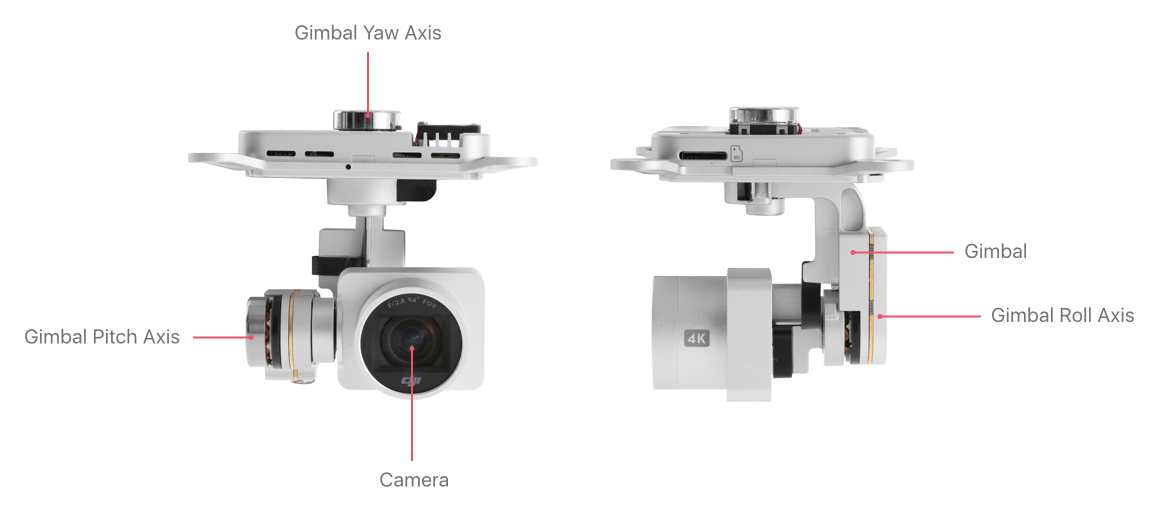
\includegraphics[width=\textwidth]{literature_review/roll_pitch_yaw_gimbal.png}
  \caption{\label{fig:roll_pitch_yaw_camera} An illustration of the roll, pitch and yaw axis used in a gimbal~\cite{roll_pitch_yaw_camera}.}
\end{figure}

While gimbal designs are fairly standard, a few critical design choices must be made when building or buying one. The rest of this chapter will detail some of the options available.

\subsection{Comparison of actuator types}
The type of actuator used in the gimbal has a significant effect on the design of the gimbal, the speed it can move, the camera weight it can handle and quality of the resulting photos and videos. Thus, a few relevant actuator types were considered and compared. A summary of their relevant characteristics can be found below, in table \ref{table:gimbal_actuators}. Note that because there are a large number options for each actuator type, some of the metrics are more qualitative/comparative than strictly quantitative. The comparisons have been made for actuators which are of the size and cost required by the project.
\newline

% TODO: finish this table

\begin{table}[h!]
	\centering
	\begin{tabular}{ p{2cm}||p{4cm}|p{4cm}|p{4cm} }
					& DC motor			& Servo motor		& BLDC \\
	\hline \hline
	Length			& $\approx 45mm$	& $\approx XXmm$	& $<30mm$ \\
	\hline
	Diameter		& XX				& XX				& $<30mm$ \\
	\hline
	Weight			& XX				& XX				& light, but requires ESC \\
	\hline
	Complexity		& moderate (H-bridge) & simple (built in) & difficult (requires PID controller) \\
	\hline
	Circuitry required & H-bridge		& None (built in)	& Requires ESCs \\
	\hline
	Efficiency		& low				& low				& high \\
	\hline
	Speed			& low				& low				& high \\
	\hline
	Price			& moderate			& low/moderate		& high \\
	\hline
	Smoothness		& moderate			& low				& very high \\
	\hline
	\end{tabular}
	\caption{Comparison of gimbal actuators}
	\label{table:gimbal_actuators}
\end{table}

To summarize the main highlights from table \ref{table:gimbal_actuators}: DC motors are a poor choice for a system of this type because most options tend to be too long and heavy, or require complex gearing. Servo motors are not a good fit because, while they're easy to use (they're essentially a DC motor with circuitry built in) and have good torque, they're fairly large and are quite jittery.

This leaves BLDC motors. While they can be quite complex to use and are somewhat expensive, they're compact, fast and tend to result in very smooth footage. As a result, they are the industry standard in camera gimbals. It is worth noting that, while the gimbal controller can be fairly complex, using a store-bought controller allows for one to easily leverage off the design work of other engineers. This results in a faster, smoother and more stable gimbal than one could build in a short period of time.

\subsection{Gimbal design inspirations}
It is useful to review existing gimbal designs in order to avoid unnecessary re-invention of the wheel. Luckily, a large number of designs are available on the internet. One design which stood out was \href{https://www.thingiverse.com}{thingiverse.com} member Velocirotor's clever gimbal design, dubbed the \href{https://www.thingiverse.com/thing:2804872}{Primbal Session} \cite{website:primbal_session}. It is a light-weight, simple to print and adjustable 3-axis gimbal for a single GoPro Hero Session. A render of the design can be found in Figure~\ref{fig:primbal_pic}.

\begin{figure}[h!]
  \centering
  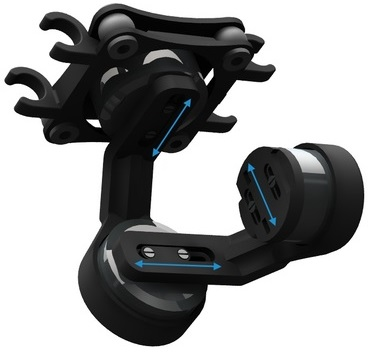
\includegraphics[width=0.5\textwidth]{literature_review/primbal_pic.jpg}
  \caption{\label{fig:primbal_pic} Render of the Primbal Session gimbal design.}
\end{figure}

Some inspiration was also taken from a gimbal designed by mechatronics engineering student Sylvan Morris, during a period of vac work. Noteworthy characteristics include the two-plate shock absorption system and method of mounting onto a quadcopter. A photo of his design can be found in Figure~\ref{fig:sylvan_gimbal}.

\begin{figure}[h!]
  \centering
  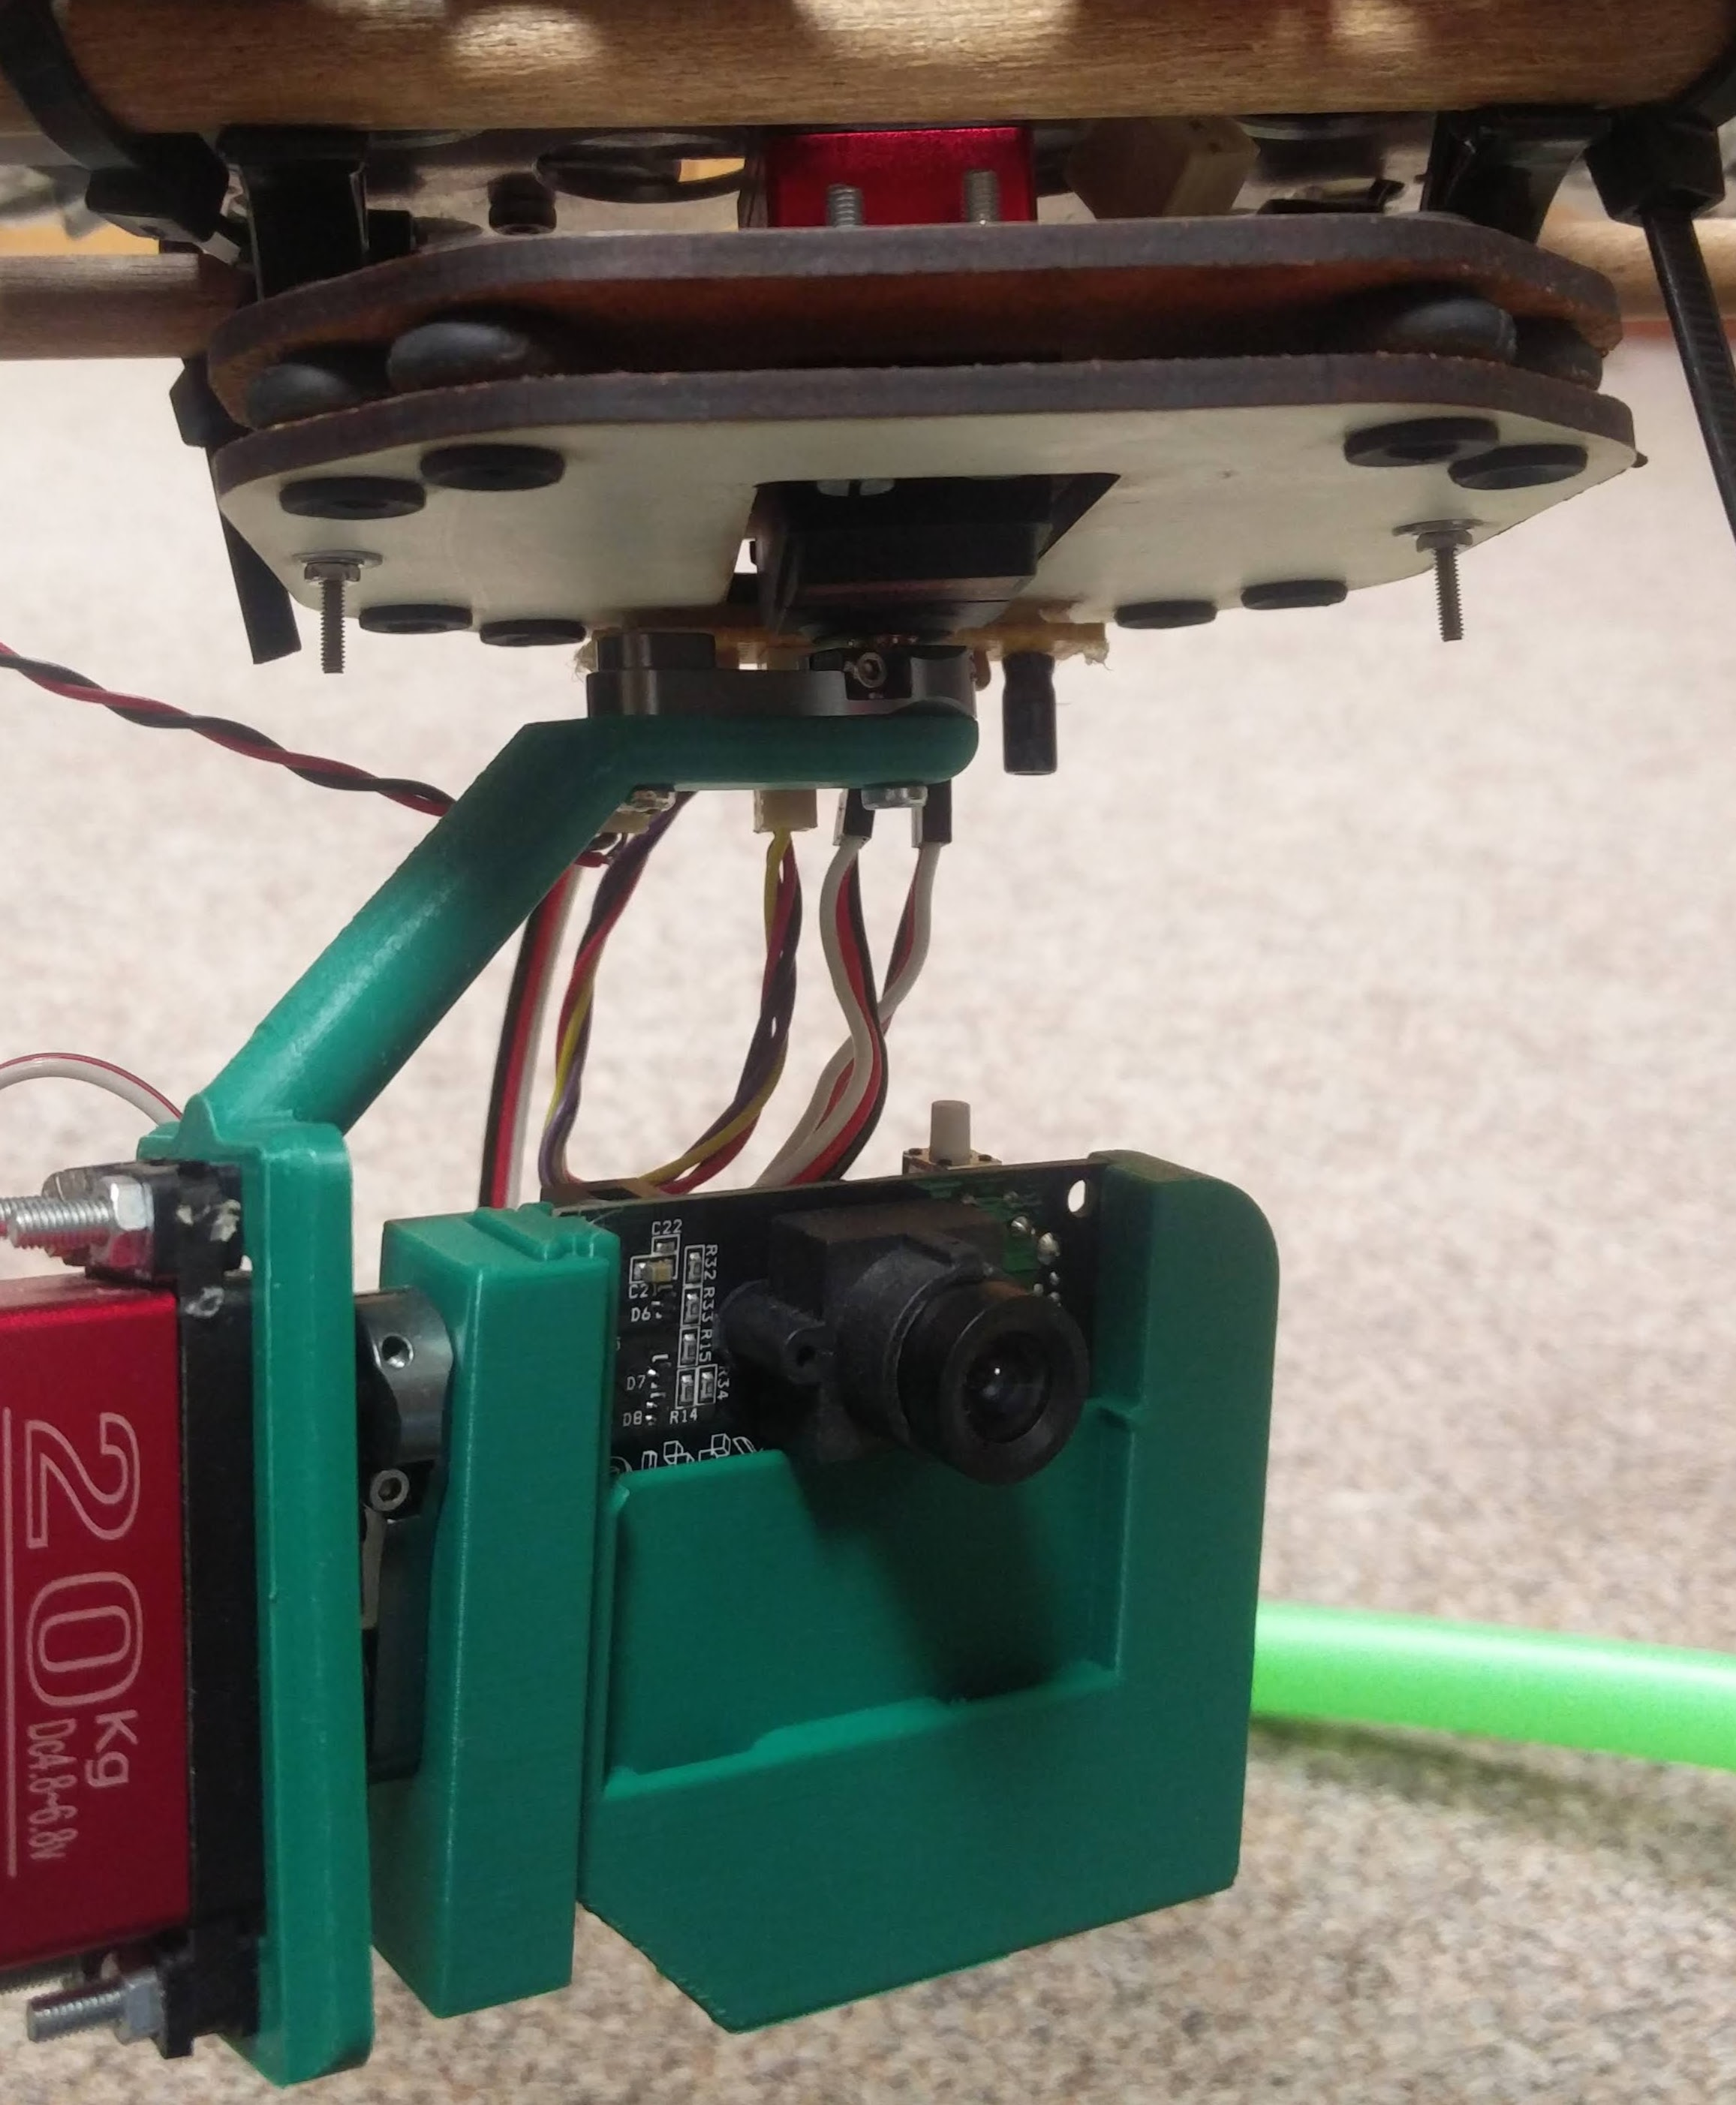
\includegraphics[width=0.5\textwidth]{literature_review/sylvan_gimbal.jpg}
  \caption{\label{fig:sylvan_gimbal} Photo of Sylvan Morris's gimbal design.}
\end{figure}

